\section[svm]{Support Vector Machines / Kernel Trick}

\begin{frame}
    \frametitle{Support Vector Machines}
    \begin{center}
        \begin{itemize}
            \item Maximum margin classifier
            \item Quadratic problem $\rightarrow$ can be solved efficiently in $O(N^2)$
            \item Optimal for linearly separable problems
            \item Slope variables allow for misclassification
        \end{itemize}

        \begin{tikzpicture}
            \node[anchor=south west,inner sep=0] (image) at (0,0) {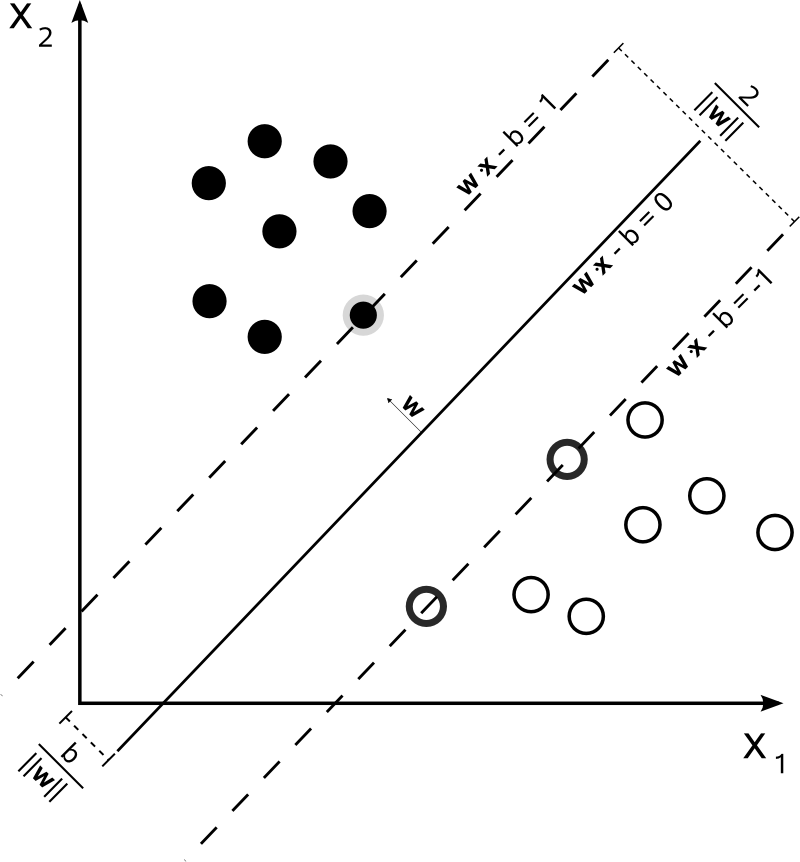
\includegraphics[width=0.4\textwidth]{svm-hyperplane.png}};
        \end{tikzpicture}
    \end{center}
\end{frame}

\begin{frame}
    \frametitle{Kernel Trick}
    \begin{center}
        \begin{itemize}
            \item SVM Algorithm depends only on scalar product!
            \item Replace scalar product with an arbitrary kernel function
            \item Solves problem in implicitly high-dimensional space
        \end{itemize}
        \begin{align*}
            \max g(c_1, \dots, c_n) = \sum_i c_i - \frac{1}{2} \sum_i \sum_j y_i c_i (\vec{x}_i \cdot \vec{x}_j) y_j c_j
        \end{align*}
    \end{center}
\end{frame}

\begin{frame}
    \frametitle{Kernel trick}
    \begin{center}
        \begin{tikzpicture}
            \node[anchor=south west,inner sep=0] at (3,0) {Linear $k(\vec{x}_i, \vec{x}_j) = \vec{x}_i \cdot \vec{x}_j$};
            \node[anchor=north west,inner sep=0] at (3,0) {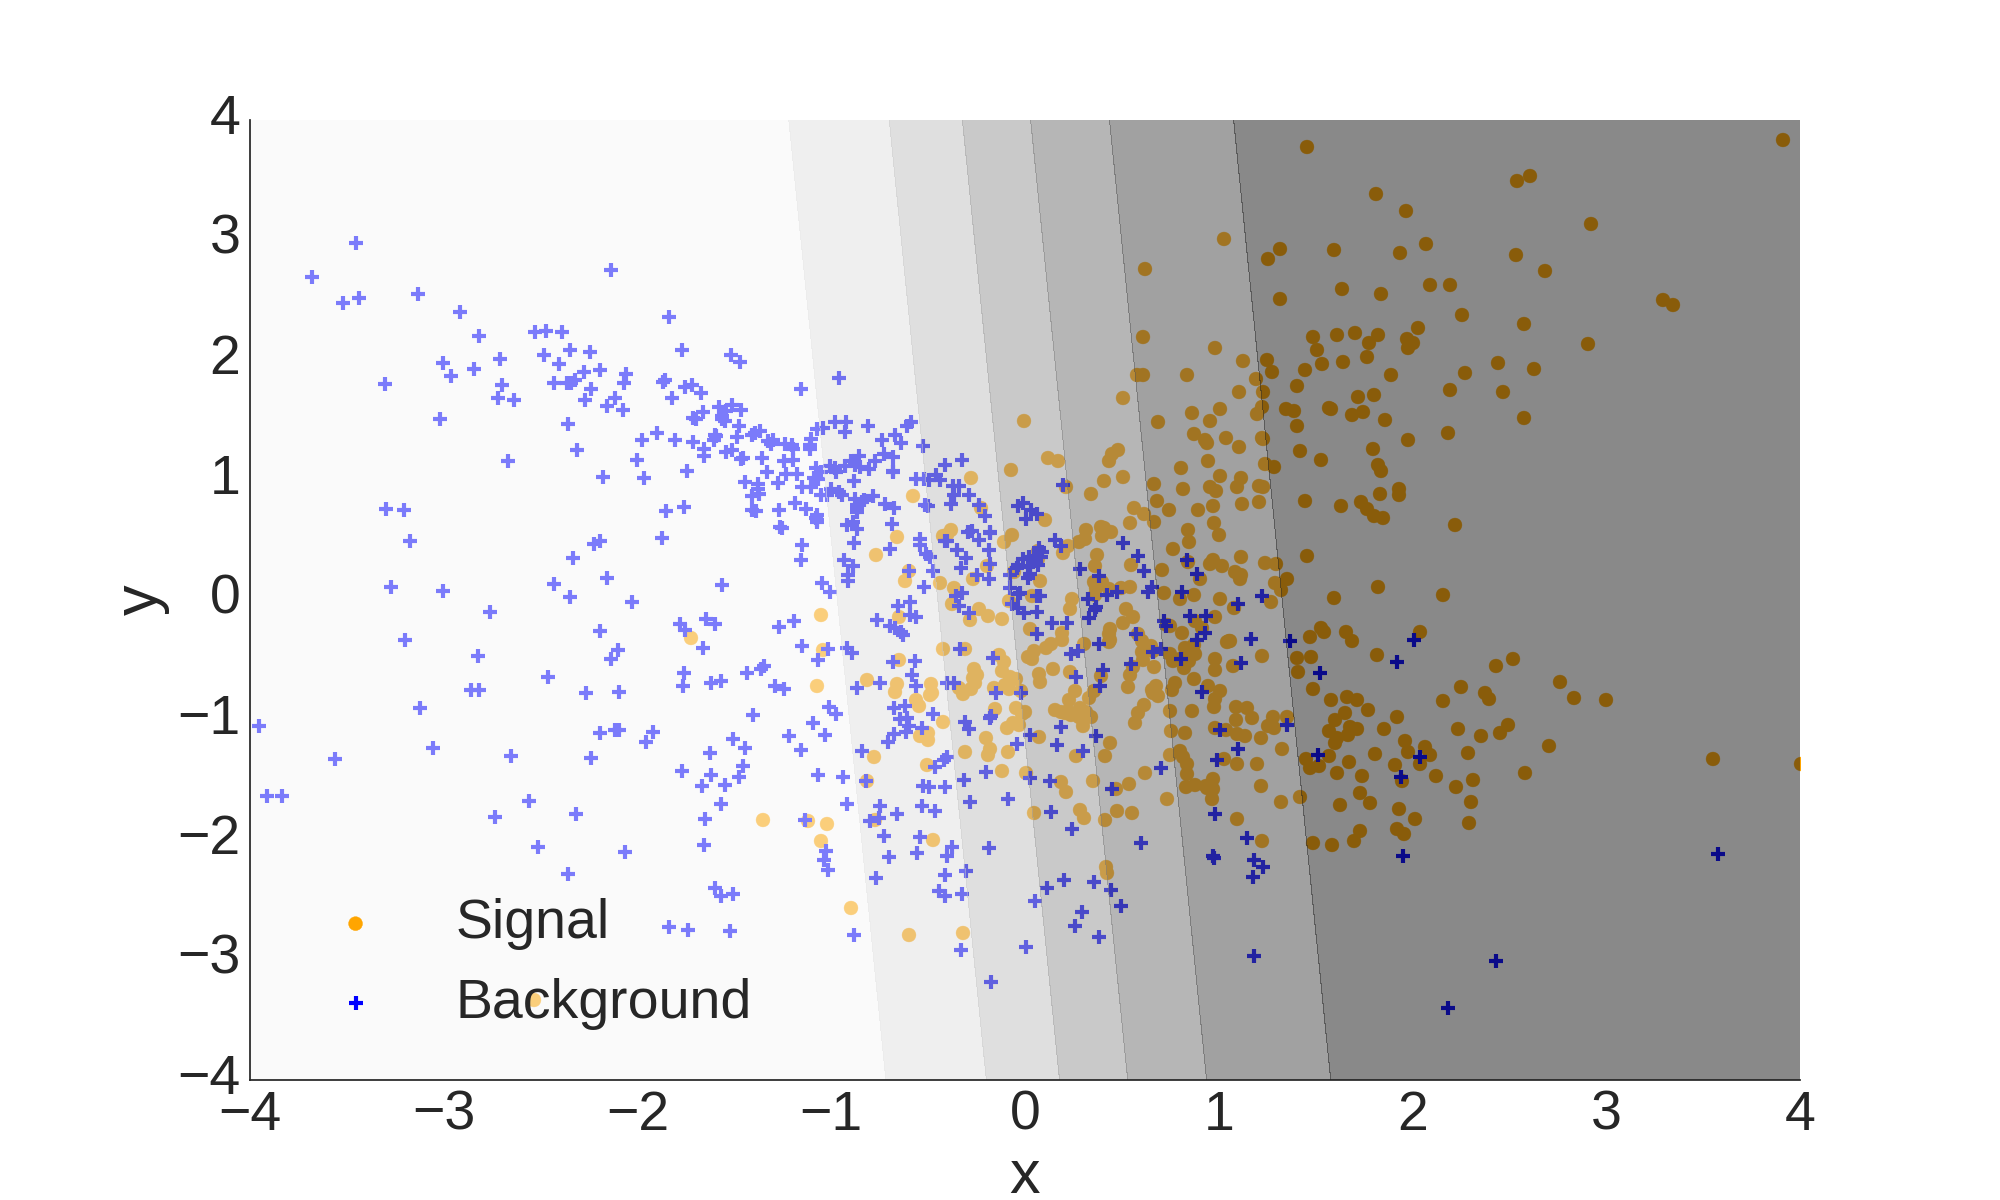
\includegraphics[width=0.4\textwidth]{linear_svm_classifier.png}};
            \node[anchor=south west,inner sep=0] at (0,-3.5) {Gausian $k(\vec{x}_i, \vec{x}_j) = \exp(- \gamma || \vec{x}_i - \vec{x}_j||^2)$};
            \node[anchor=north west,inner sep=0] at (0,-3.5) {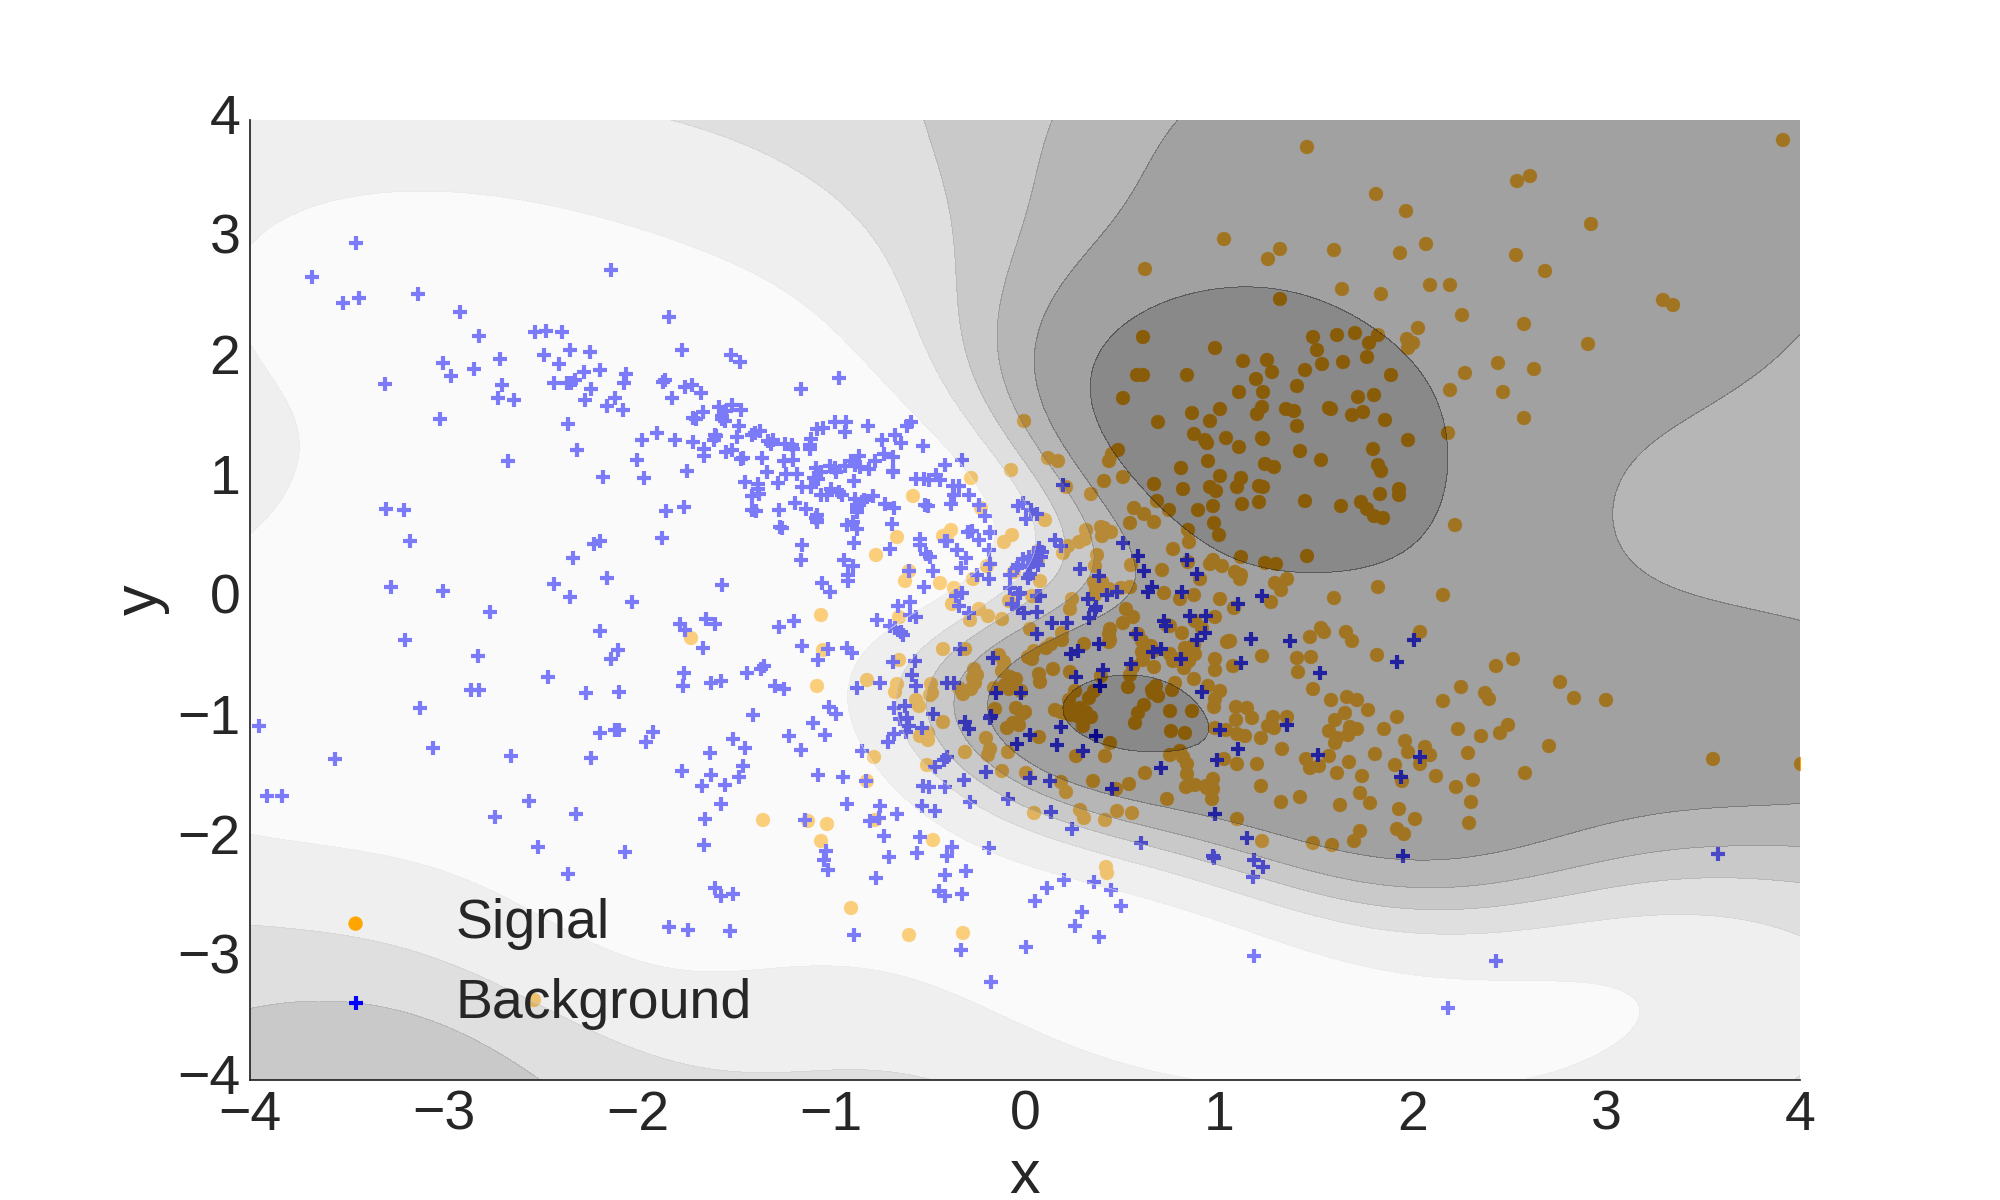
\includegraphics[width=0.4\textwidth]{rbf_svm_classifier.png}};
            \node[anchor=south west,inner sep=0] at (6,-4.2) {Polynomial $k(\vec{x}_i, \vec{x}_j) = (\vec{x}_i \cdot \vec{x}_j)^d$};
            \node[anchor=north west,inner sep=0] at (6,-4.2) {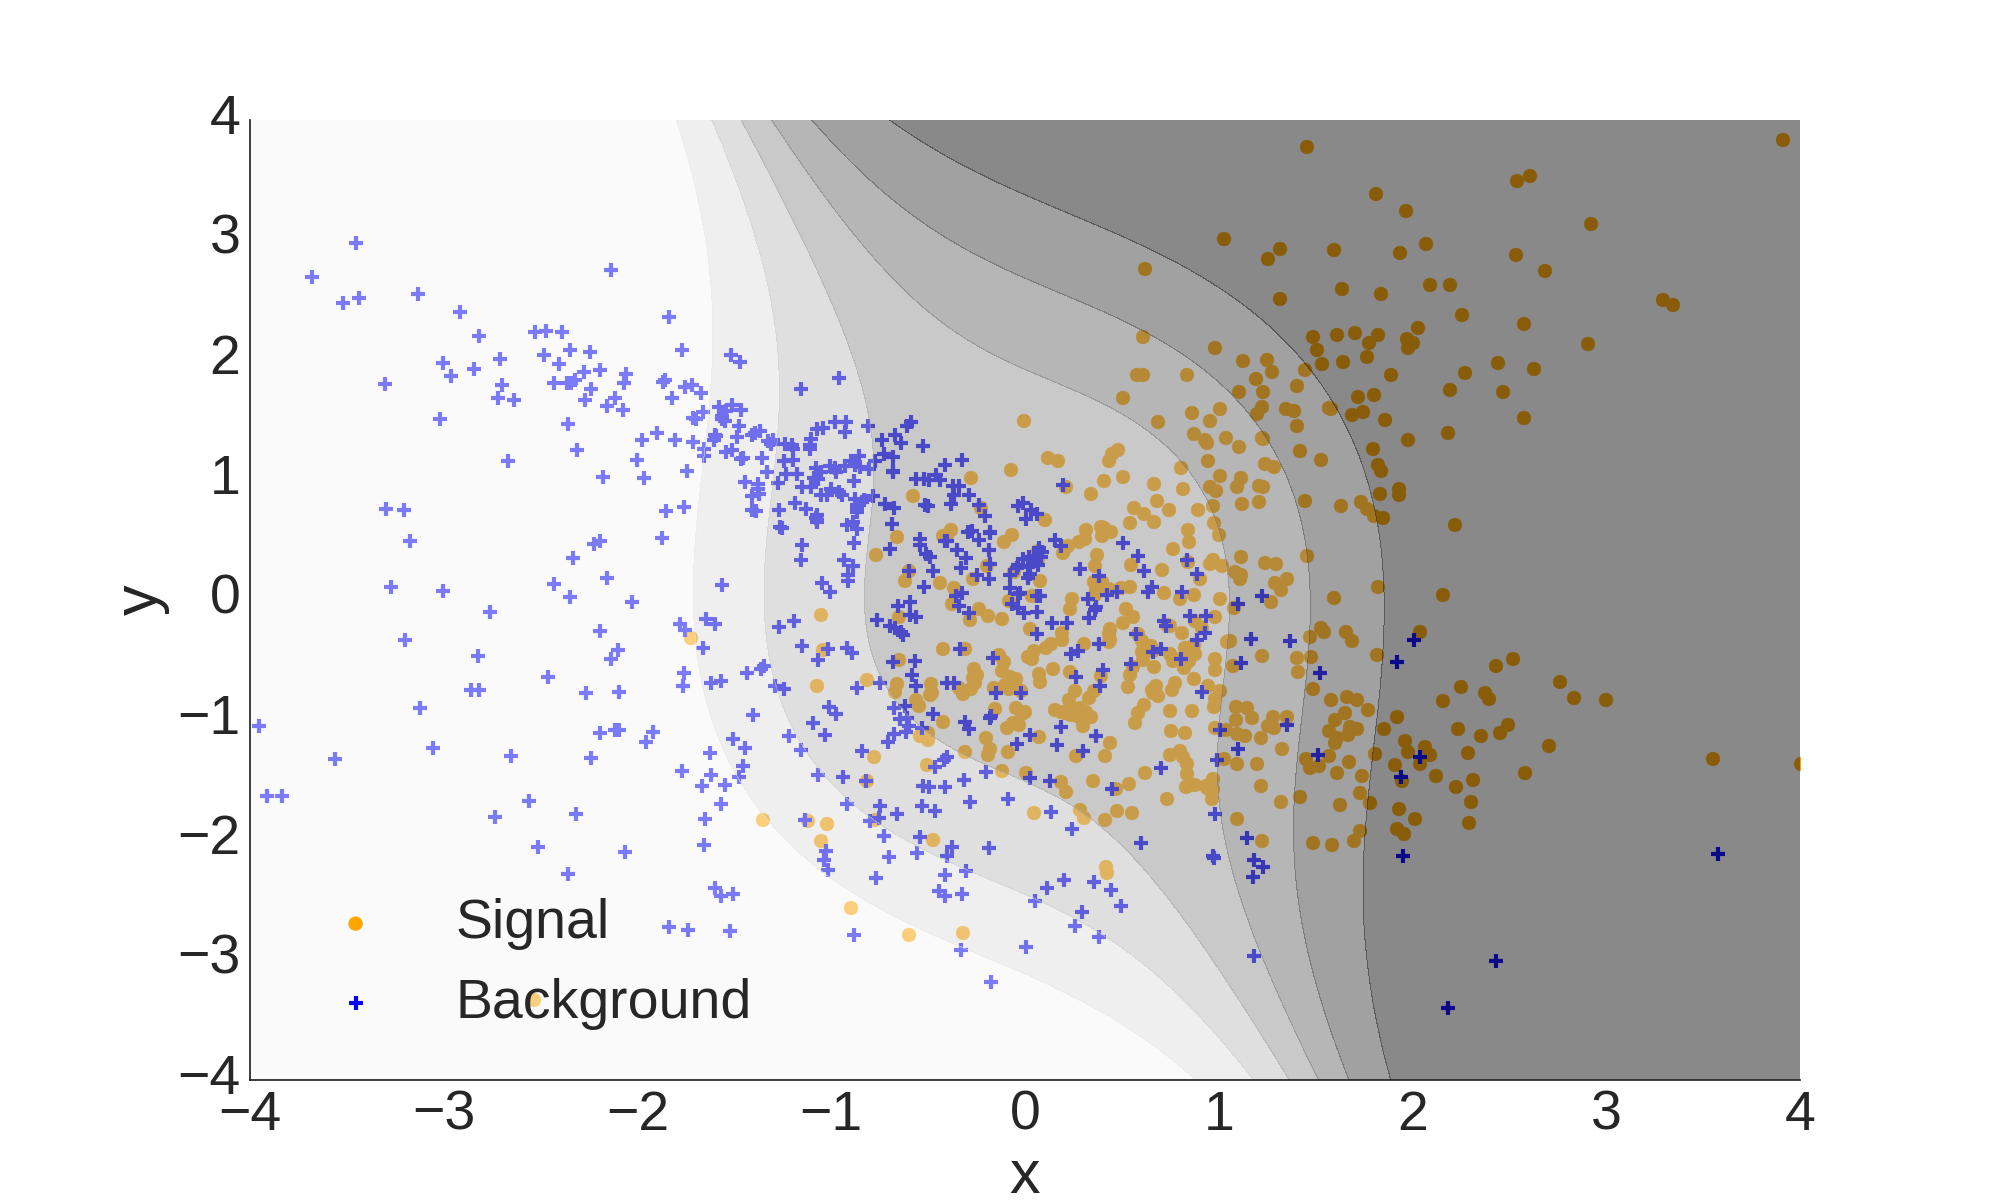
\includegraphics[width=0.4\textwidth]{poly_svm_classifier.png}};
        \end{tikzpicture}
    \end{center}
\end{frame}

\begin{frame}
    \frametitle{Example Classifier Quality}
    \begin{center}
        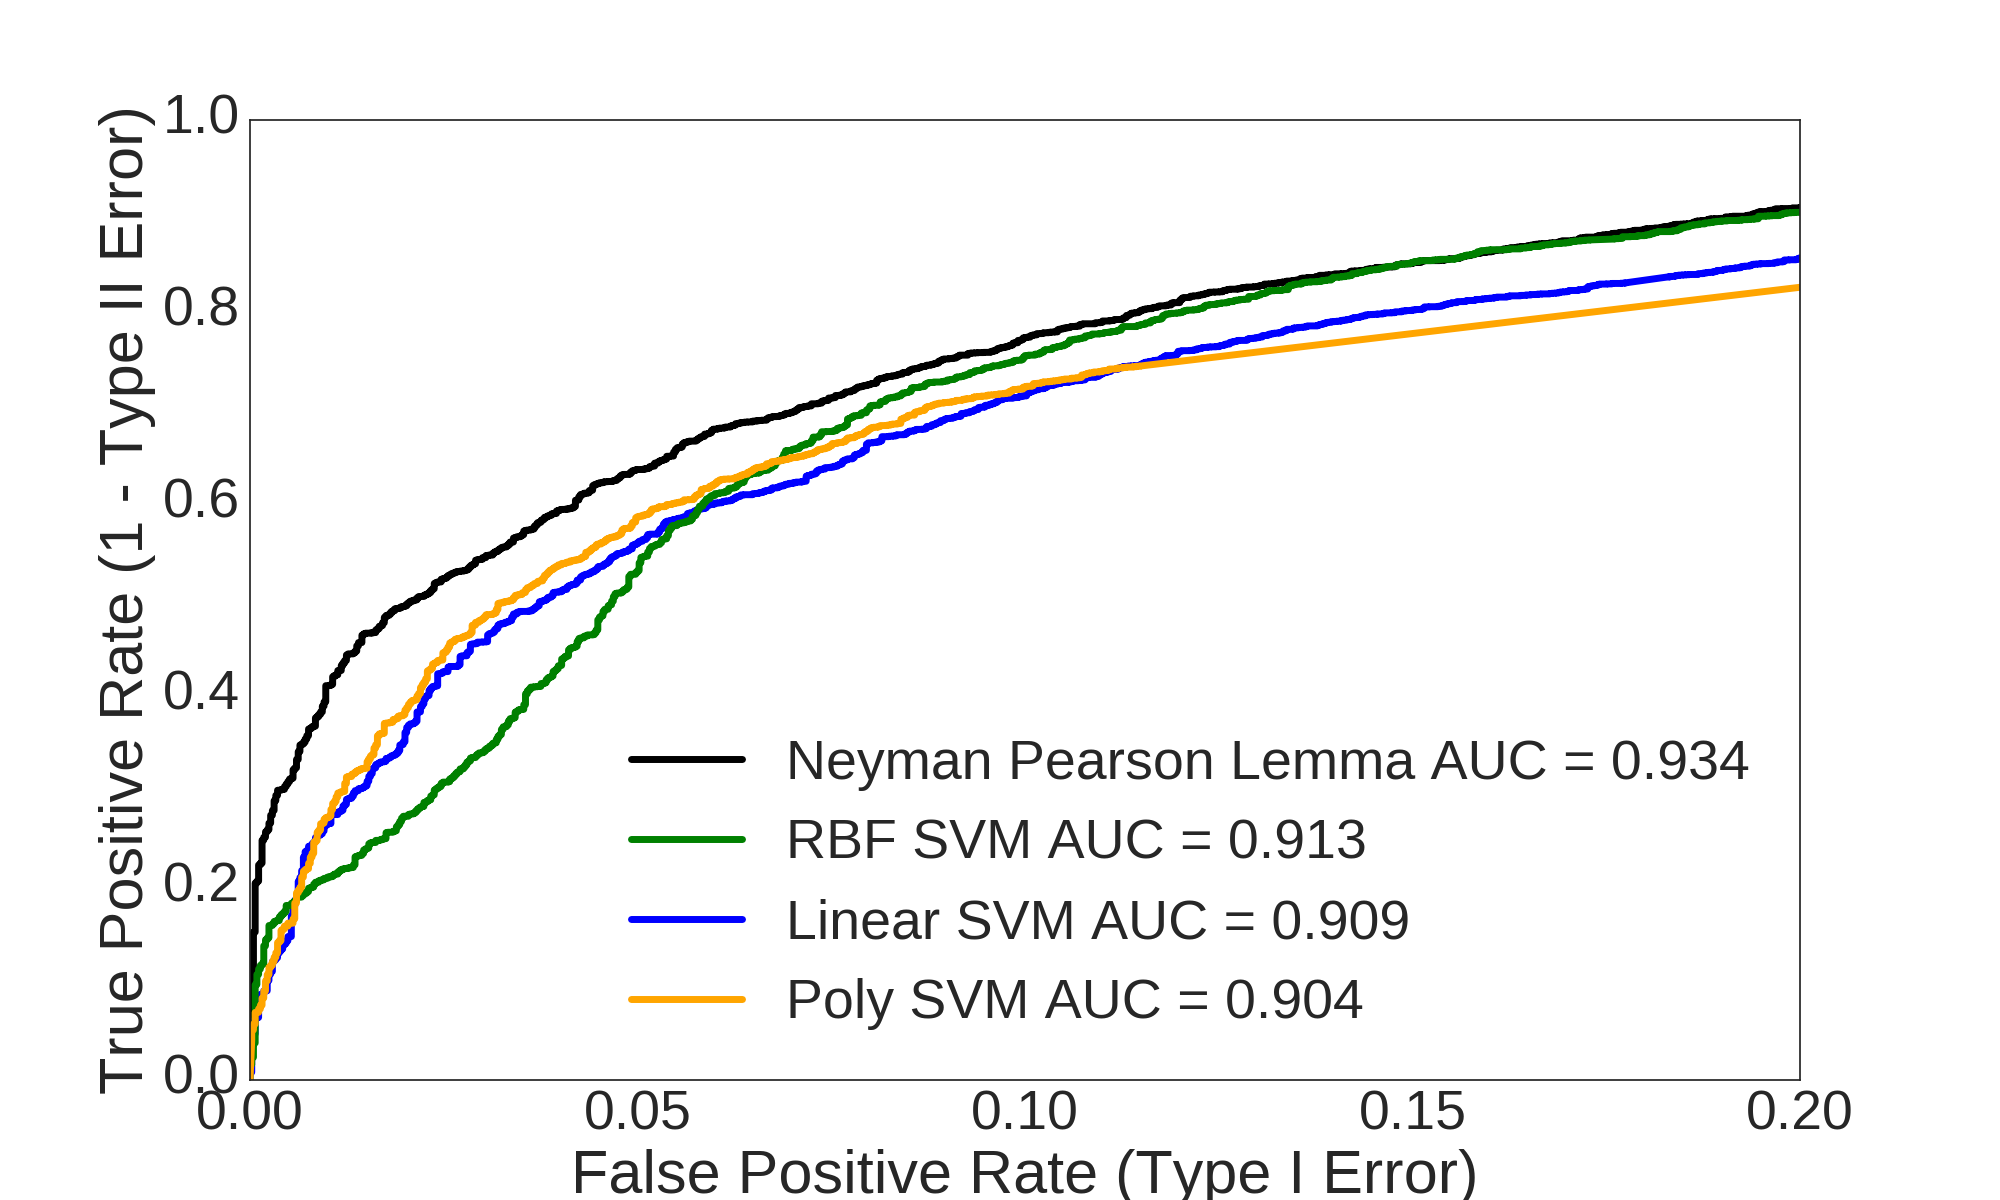
\includegraphics[width=\textwidth]{svm_roc.png}
    \end{center}
\end{frame}
